\begin{tikzpicture}
    \node                         (mix) at (0, 1) {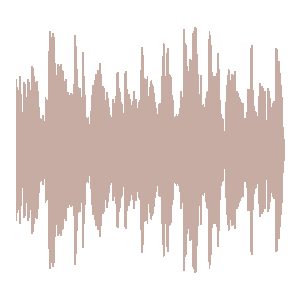
\includegraphics[width=30pt]{wave/mix}};
    \node[right=10pt of mix,draw] (aprxpost)      {\(\aprxpost\)};

    \draw[->] (mix) -- (aprxpost);

    % Mix wave
    \node[right=125pt of aprxpost, yshift=-61pt] (sum) {\(+\)};
    \node[right=-8pt of sum] (wav) {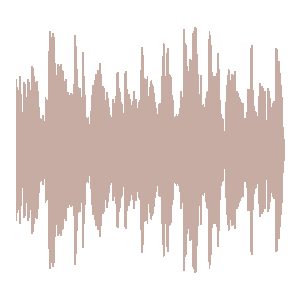
\includegraphics[width=30pt]{wave/mix}};

    % Langevin
    \node[below right=90pt and -5pt of aprxpost] (lstart) {};
    \node[below left=25pt and 20pt of wav] (lend) {};
    \draw[->] (lstart) .. controls ([yshift=-1cm, xshift=1cm,] lstart) and ([xshift=-1cm, yshift=-1cm] lend) .. node[below] {sampling} node[above] {Langevin} (lend);
    %\draw[->, bend angle=90, bend right=100]  (lstart) -- node[below] {sampling} node[above] {Langevin} (lend);

    \foreach \source/\offset in {other/0,drums/1,voice/2,bass/3}{%
    \begin{scope}
        \node    (stem) at (0, -0.75*\offset)   {\includegraphics[width=20pt]{musdb/\source.png}};
        \node[right=10pt of stem,draw] (flow)   {\(p(\s_k)\)};
        \node[right=10pt of flow]      (prior)  {\includegraphics[width=25pt]{dist/\source}};
        \draw[->] (stem) -- (flow);
        \draw[->] (flow) -- (prior);
        \node[right=70pt of prior]  (sample) {\includegraphics[width=25pt]{wave/\source}};
        % \draw[->, bend angle=-45, bend right=-70] (prior.center) to (sample.west);
        \draw (sample) -| (sum);


        \node[right=20pt of prior] (post)   {\includegraphics[width=25pt]{dist/\source_post}};
        \draw[densely dotted, bend right=20] ([shift={(-0.1, -0.3)}]post.center) to ([shift={(0.05, -0.05)}]prior.center);
        \draw[densely dotted, bend right=20] ([shift={(-0.2, 0.15)}]post.center) to ([shift={(0.05, 0.05)}]prior.center);
        \draw[->] (post) -- (sample);
        \draw[->, bend angle=90, bend right=-120] (aprxpost.east) to ([xshift=-10]post.east);
    \end{scope}}%

\end{tikzpicture}

% \begin{tikzpicture}
%     % Data column
%     \node                  (s0) {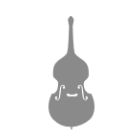
\includegraphics[width=25pt]{mixing/bass.png}};
%     \node[below=0pt of s0] (s1) {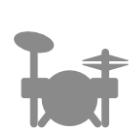
\includegraphics[width=25pt]{mixing/drums.png}};
%     \node[below=0pt of s1] (s2) {
\includegraphics[width=25pt]{mixing/voice.png}};
%     \node[below=0pt of s2] (s3) {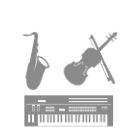
\includegraphics[width=25pt]{mixing/other.png}};

%     % Prior column
%     \node[right=50pt of s0] (d0) {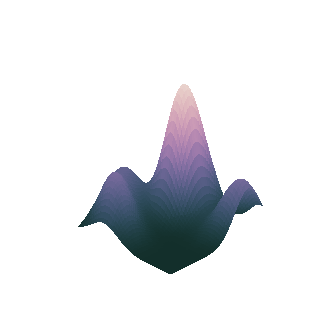
\includegraphics[width=40pt]{dist_0}};
%     \node[right=50pt of s1] (d1) {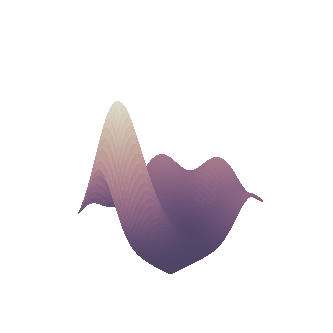
\includegraphics[width=40pt]{dist_1}};
%     \node[right=50pt of s2] (d2) {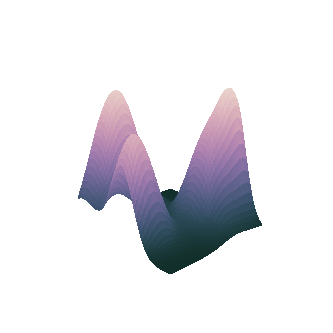
\includegraphics[width=40pt]{dist_2}};
%     \node[right=50pt of s3] (d3) {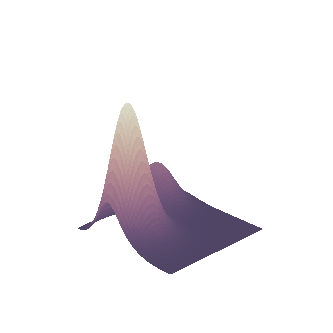
\includegraphics[width=40pt]{dist_3}};

%     % Data to prior arrows
%     \draw[->] (s0) to (d0);
%     \draw[->] (s1) to (d1);
%     \draw[->] (s2) to (d2);
%     \draw[->] (s3) to (d3);

%     % Posterior column
%     \node[right=20pt of d0] (dp0) {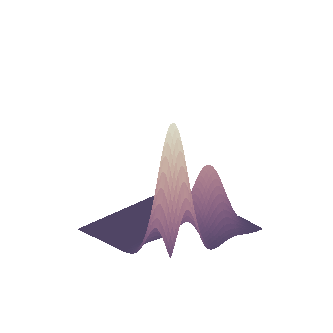
\includegraphics[width=40pt]{dist_0_post}};
%     \node[right=20pt of d1] (dp1) {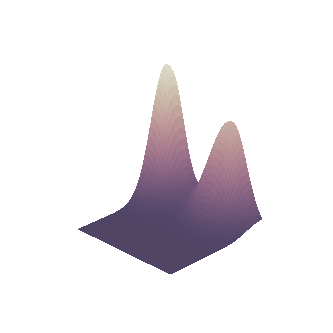
\includegraphics[width=40pt]{dist_1_post}};
%     \node[right=20pt of d2] (dp2) {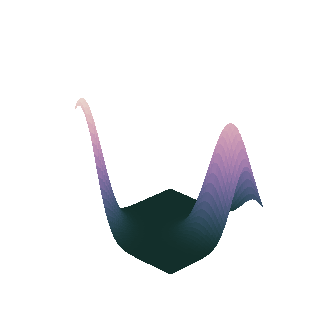
\includegraphics[width=40pt]{dist_2_post}};
%     \node[right=20pt of d3] (dp3) {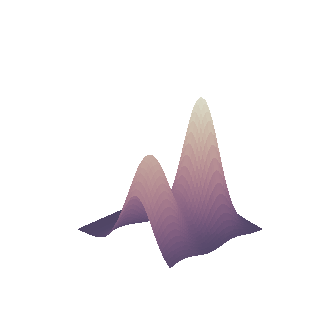
\includegraphics[width=40pt]{dist_3_post}};

%     % Sample column
%     \node[right=30pt of dp0] (ps0) {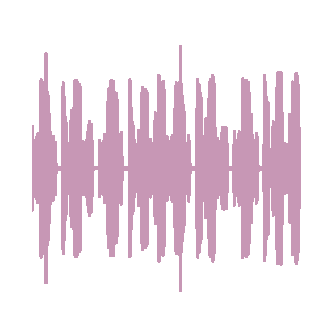
\includegraphics[width=30pt]{wave_bass}};
%     \node[right=30pt of dp1] (ps1) {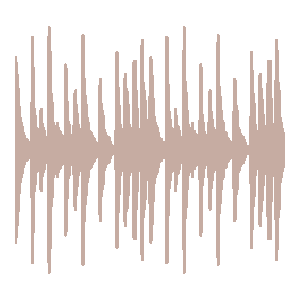
\includegraphics[width=30pt]{wave_drums}};
%     \node[right=30pt of dp2] (ps2) {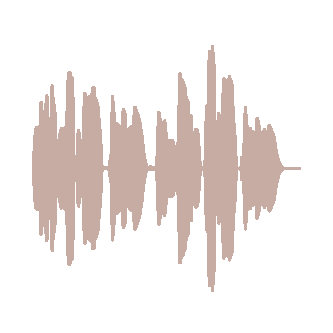
\includegraphics[width=30pt]{wave_voice}};
%     \node[right=30pt of dp3] (ps3) {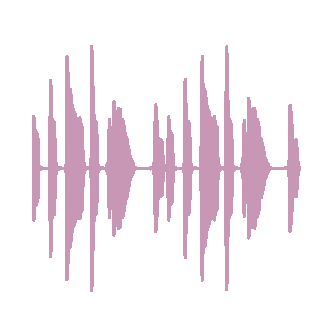
\includegraphics[width=30pt]{wave_other}};

%     % Arrows from posterior to samples
%     \draw[->] (dp0) to (ps0);
%     \draw[->] (dp1) to (ps1);
%     \draw[->] (dp2) to (ps2);
%     \draw[->] (dp3) to (ps3);

%     % Top row, notes
%     \node[above=0pt of s0]   (ts)  {\(\D_k\)};
%     \node[above=-9pt of d0]  (td)  {\(p_{\B{\θ}}(\s_k)\)};
%     % \path (ts) -- (td) node [midway,align=center] {estimate\\with flow};
%     \node[above=-9pt of dp0] (tdp) {\(\aprxpost\)};
%     \node[above=0pt of ps0]  (tps) {\(\s_k\)};

%     % Top top row
%     \node[above=0pt of ts]  () {data};
%     \node[above=0pt of td]  () {prior};
%     \node[above=0pt of tdp] () {posterior};
%     \node[above=0pt of tps] () {sample};

%     % Mix wave
%     \node[right=5pt of ps1, yshift=-20pt] (sum) {\(+\)};
%     \node[right=-8pt of sum] (wav) {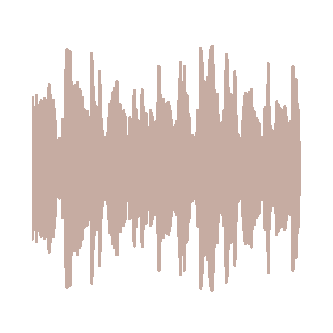
\includegraphics[width=30pt]{wave_mix}};

%     \draw (ps0) -| (sum)
%           (ps1) -| (sum)
%           (ps2) -| (sum)
%           (ps3) -| (sum);

%     % Langevin
%     \draw[->, bend angle=45, bend right=40]  ([yshift=-5pt]d3) to node[below] {sampling} node[above] {Langevin} ([yshift=-12pt,xshift=-10pt]ps3);
% \end{tikzpicture}
